\section{Realizzazione}
\subsection{Gerarchia dei File}
nella cartella principale \textit{Webpage} sono contenuti i file php che contengono la struttura del sito e 4 cartelle:
\begin{itemize}
	\item \textbf{general:} contiene parti della strutturo del sito che sono presenti in più pagine;
	\item \textbf{images:} contiene tutte le immagini presenti nel sito;
	\item \textbf{php-script} contiene tutti i file che contengono varie funzioni utili al funzionamento del sito;
	\item \textbf{style:} contiene tutti i file css che modellano la presentazione del sito.
\end{itemize}
\subsection{Struttura}
La pagina e' stata scritta in HTML 5, la struttura del sito con questo standard non è moto diversa da come sarebbe stata con XHTML ma introduce dei tag semantici che abbiamo utilizzato come \emph{section}.\newline
Il sito e' composto da pagine php che hanno la funzione di produrre dinamicamente il codice html che verrà letto dai browser.\newline
In questa sezione sono inserite alcune immagini di parti del sito che abbiamo ritenuto fondamentali per l'esperienza dell'utente, alcune immagini non sono state inserite perché ritenute troppo simili ad altre già inserite. 


\subsubsection{Barra di navigazione} 
Ogni pagina ha una barra di navigazione, le voci presenti in questa barra variano a seconda del tipo di utente che sta visitando la pagina.
\begin{itemize}
\item Se l'utente non è autenticato vedrà le voci home, prodotti, login e registrati;
\item Se l'utente è registrato vedrà le voci home, prodotti, account, carrello e logout;
\item se l'utente è un admin vedrà le voci home, prodotti , account, gestione sito e logout.
\end{itemize}
grazie a questa barra di navigazione è possibile accedere a tutte le pagine che servono all'utente per navigare nel sito e all'amministratore per gestirlo. Oltre alle voci in questa barra è presente una barra di ricerca, inserendo una parola chiave questa viene cercata all'interno del nome del tipo e della descrizione dei prodotti presenti nel sito e l'utente viene indirizzato alla pagina dei prodotti contenente solamente i prodotti cercati.
\begin{figure}[h]
	\label{navbarz} 
	\centering 
	
\includegraphics[width=1\textwidth]{immagini/navbar.png}
	\caption{Esempio di barra di navigazione per utenti non autenticati} 
\end{figure}

\subsubsection{Home}
La home è composta da due sezioni:
\begin{itemize}
	\item La sezione dei bundle proposti dal sito che sono tre(High,Medium,Low) divisi per fasce di prezzo, ognuno di questi è un insieme di pezzi che compongono un pc, nella schermata home però ne viene visualizzato solo una breve descrizione e il nome dal quale si potrà accedere alla pagina del bundle specifico.
	\item La sezione best sellers mostra i tre pezzi più venduti, per ciascuno di questi prodotti vengono visualizzati nome, categoria, valutazione, prezzo e un'immagine, cliccando sul nome è possibile raggiungere la pagina di dettaglio del prodotto.
\end{itemize}
\begin{figure}[h!]
	\label{bundle} 
	\centering 
	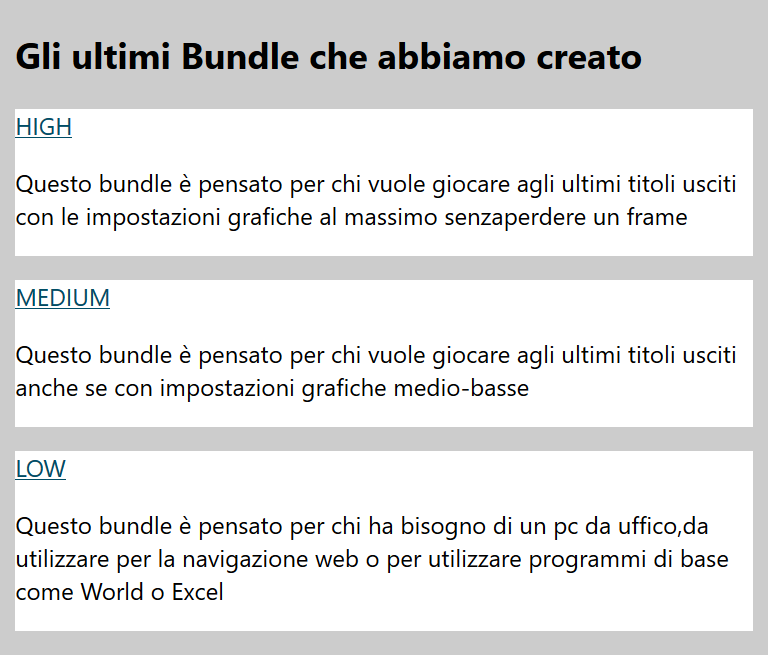
\includegraphics[width=0.6\textwidth]{immagini/Bundle.png}
	\caption{Sezione bundle nella schermata home} 
	\mbox{} \\
\end{figure}
\begin{figure}[h!]
	\label{bs} 
	\centering 
	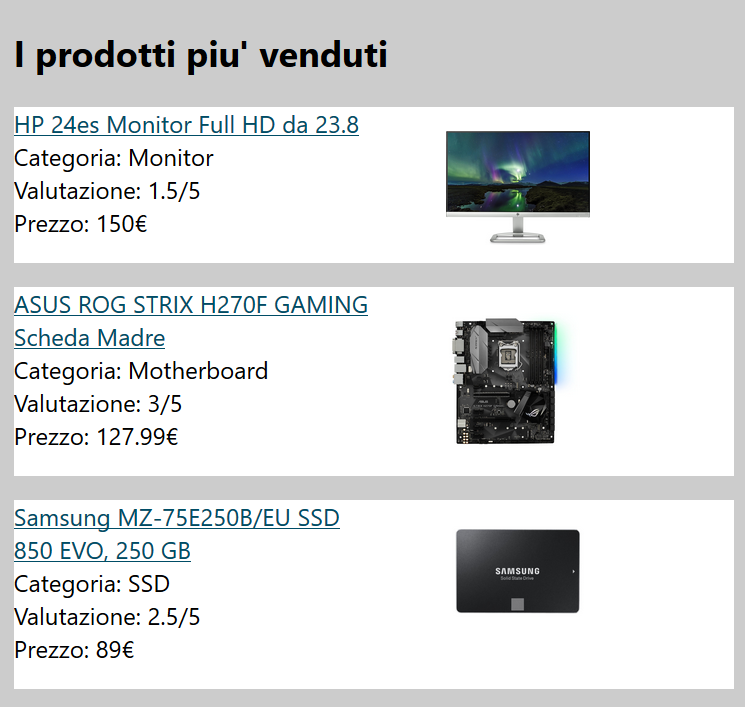
\includegraphics[width=0.6\textwidth]{immagini/bs.png}
	\caption{Sezione best seller nella schermata home} 
\end{figure}
\mbox{} \\

\subsubsection{Prodotti}
La pagina dei prodotti mostra tutti i prodotti presenti nel sito sotto forma di lista, è stata scelta una lista piuttosto che una tabella per una questione di accessibilità infatti i contenuti sono più leggibili e lo rimangono su schermi più piccoli come quelli degli smartphone.\newline
Per ogni prodotto viene visualizzato nome, categoria, descrizione parziale(i primi 200 caratteri), valutazione, prezzo e una immagine, da questa pagina viene inoltre fornita la possibilità di andare alla pagina di dettaglio del prodotto cliccando su vai al dettaglio oppure sul nome del prodotto.\newline
In questa pagina inoltre è possibile effettuare una ricerca avanzata selezionando la categoria del prodotto e il tipo di ordinamento che si vuole per la lista. \mbox{} \\ \mbox{} \\ \Spazio

\begin{figure}[h!]
	\label{prodotti} 
	\centering 
	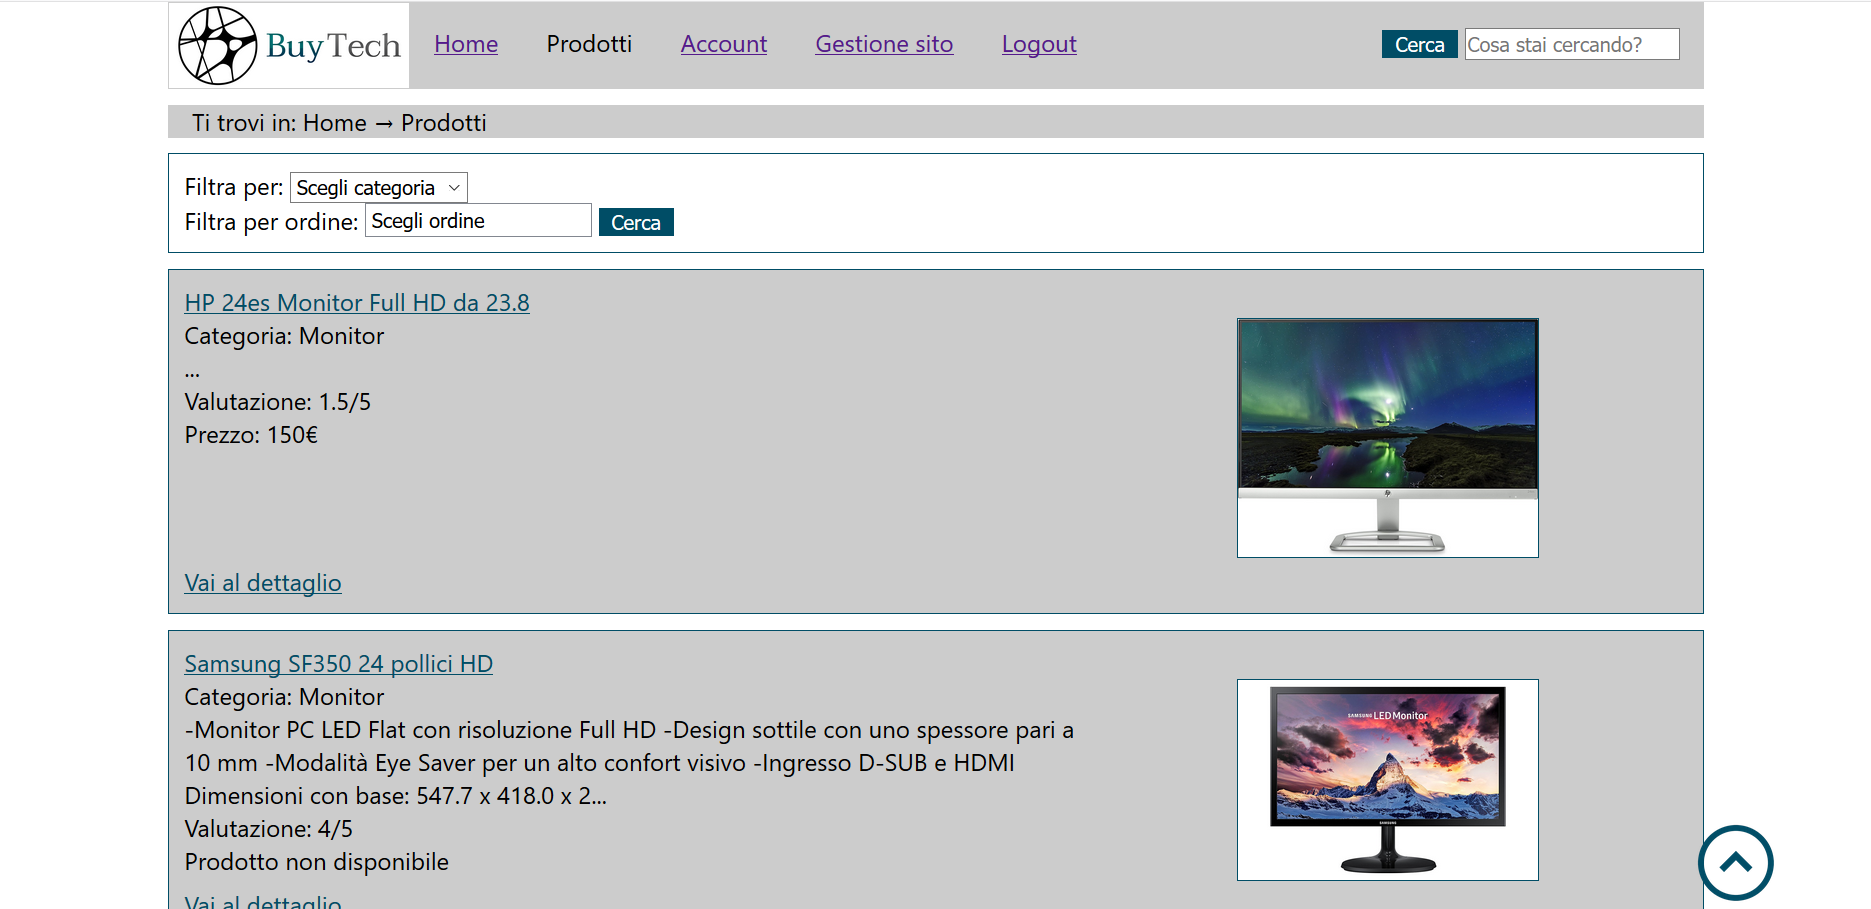
\includegraphics[width=0.9\textwidth]{immagini/prodotti.png}
	\caption{pagina dei prodotti} 
\end{figure}
\mbox{} \\

\subsubsection{Dettaglio Prodotto}
La pagina di dettaglio del prodotto mostra il nome, categoria, descrizione completa, valutazione, prezzo e l'immagine di un prodotto specifico.\newline
Attraverso il pulsante \emph{Aggiungi al carrello} è possibile aggiungere il prodotto visualizzato al proprio carrello per poi procedere al suo acquisto.\newline
In questa pagina è inoltre possibile visualizzare le recensioni date da chi ha già comprato il prodotto.

\begin{figure}[h!]
	\label{dettaglio} 
	\centering 
	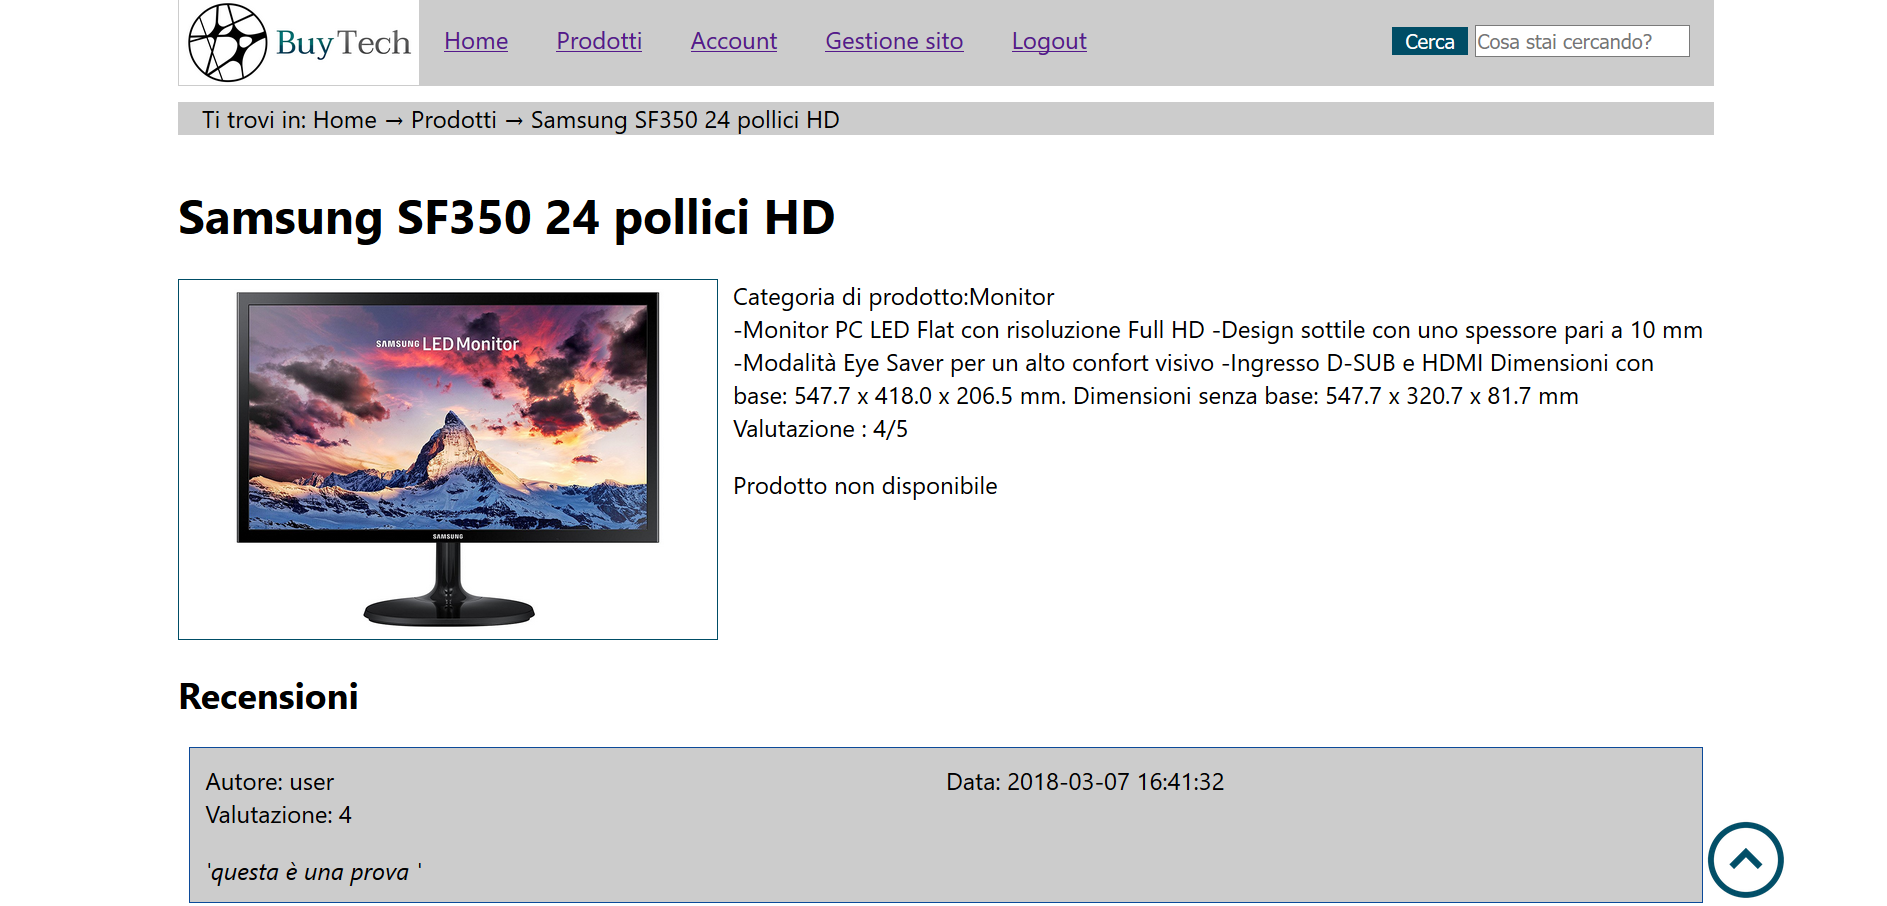
\includegraphics[width=0.9\textwidth]{immagini/dettaglio.png}
	\caption{pagina di dettaglio di un prodotto con una recensione annessa} 
\end{figure}
\mbox{} \\

\subsubsection{Login}
La pagina di login permette agli utenti non autenticati di autenticarsi e in caso non abbiano una account da la possibilità di passare alla pagina di registrazione.

\begin{figure}[h!]
	\label{login} 
	\centering 
	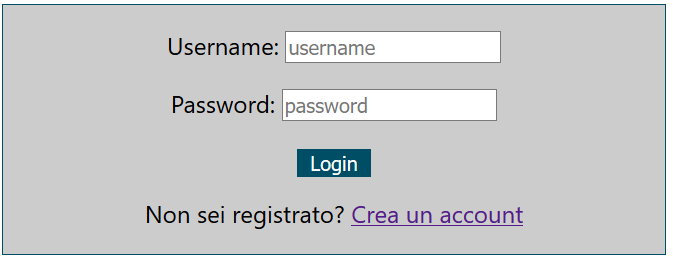
\includegraphics[width=0.6\textwidth]{immagini/login.png}
	\caption{form per la login} 
\end{figure}
\mbox{} \\

\subsubsection{Registrazione}
La pagina di registrazione da la possibilità ad un utente non registrato di registrarsi e mette in chiaro i vari vincoli sui campi da riempire.

\subsubsection{Account}
La pagina di gestione dell'account permette all'utente di visualizzare informazioni sul suo account ovvero nome utente, e-mail e data di creazione dell'account e permette di accedere allo storico degli acquisti e al carrello, permette inoltre di effettuare il logout.

\subsubsection{Carrello}
Nella pagina Carrello vengono visualizzati tutti i prodotti che sono stati selezionati dall'utente durante la sua navigazione, per ogni prodotto viene mostrato il nome, la quantità, una valutazione e il prezzo, è inoltre possibile rimuovere il prodotto dal carrello.\newline
Alla fine della lista dei prodotti del carrello viene visualizzato il prezzo totale ed è presente il tasto per acquistare il contenuto del carrello, visto che questo è un progetto didattico la gestione del pagamento non viene fatta e tutti gli articoli passano direttamente nello storico degli acquisti.

\subsubsection{Storico acquisti}
Nella pagina Storico acquisti vengono visualizzati in una lista tutti i prodotti acquistati dall'utente, per ogni prodotto viene visualizzato il nome, la categoria, una breve descrizione, la valutazione e un'immagine, inoltre cliccando sul pulsante aggiungi recensione l'utente viene indirizzato alla pagina per aggiungere una recensione al prodotto.

\subsubsection{Aggiunta recensione}
La pagina di aggiunta recensione da la possibilità di inserire una recensione di un prodotto che l'utente ha acquistato inserendo la valutazione e un testo valido che descriva l'esperienza con il prodotto.

\subsubsection{Gestione Sito}
Questa pagina è visibile solo agli admin ed ha la funzionalità di indirizzare gli admin alle pagine per apportare modifiche al sito, la pagina è composta da una lista di quattro voci:
\begin{itemize}
	\item aggiunta/modifica prodotti;
	\item gestione account;
	\item aggiunta/modifica bundle;
	\item storia degli acquisti.
\end{itemize}

\subsubsection{aggiunta/modifica prodotti}
Questa pagina è visibile solo agli admin e serve ad aggiungere al database dei prodotti oppure a modificare quelli già esistenti.\newline
L'aggiunta viene fatta tramite un form dove vanno inseriti nome,categoria, descrizione e prezzo del prodotto, l'immagine invece va inserita nella cartella images del sito con nome [id].png dove [id] è il numero identificativo del prodotto, visto che gli id sono un campo \emph{AutoIncrement} nel database basterà aggiungere uno all'id più grande.\newline
per la modifica invece bisogna cliccare il tasto modifica prodotto sulla riga della tabella del prodotto che si vuole modificare e modificare i campi del form che verrà caricato.\newline
I prodotti in questa pagina vengono visualizzati in una tabella, abbiamo fatto ciò perché secondo noi risulta più sintetica, la sua visualizzazione su mobile però non è facile da consultare comunque un admin userà il sito sempre tramite desktop e per questo abbiamo deciso di lasciare la visualizzazione dei prodotti in forma tabellare.

\subsubsection{gestione account}
In questa pagina vengono visualizzati tutti gli account presenti nel database del sito sotto forma di tabella e cliccando il tasto "cambia privilegi" è possibile far diventare un utente comune un admin e vice versa

\subsubsection{aggiunta/modifica bundle}
Questa pagina è visibile solo agli admin e serve ad aggiungere dei bundle al database oppure a modificarli o rimuoverli.
Per aggiungere bundle è presente un form nel quale va inserito il nome e la descrizione e una volta premuto il tasto crea viene data la possibilità di aggiungere i prodotti al bundle cliccando il pulsante aggiungi della riga del prodotto che si vuole aggiungere.\newline
Per modificare un bundle invece bisogna premere il tasto modifica bundle delle riga del bundle che si vuole modificare, verranno così mostrate due tabelle una per i prodotti presenti nel bundle e una per i prodotti presenti nel sito, premendo su aggiungi prodotto, i prodotti vengono aggiunti alla tabella del bundle mentre cliccando su \emph{rimuovi} questo viene tolto dal bundle.\newline
Per rimuovere un bundle basta cliccare \emph{elimina bundle} sulla tabella iniziale che mostra i nomi dei vari bundle.

\subsubsection{Storico acquisti globale}
Questa pagina è visibile solo agli admin e mostra tutti gli acquisti effettuati sul sito sotto forma di tabella, le informazioni riportate sono:
\begin{itemize}
	\item compratore;
	\item nome prodotto;
	\item categoria prodotto;
	\item valutazione;
	\item Id del prodotto;
	\item data e ora dell'acquisto.
\end{itemize}
